\chapter{\IfLanguageName{dutch}{Literatuurstudie}{Literature review}}%
\label{ch:literatuurstudie}

\section{\IfLanguageName{dutch}{Stand van zaken}{State of the art}}%
\label{sec:state-of-the-art}

Om informatie te verkrijgen, onderscheiden veel studenten twee belangrijke informatiebronnen: bronnen afkomstig van de hogeschool en informatie uitgewisseld door studenten zelf.

Vanuit de hogeschool worden verschillende informatiebronnen aangeboden waarop studenten en docenten antwoorden kunnen vinden op hun vragen. Ten eerste zijn er de inleidende slides van het vak. Hierin is informatie te vinden over eventueel aan te schaffen materialen, mogelijke softwarevereisten, deadlines en de organisatie van het vak. Naast de inleidende slides zijn er de gewone slides, die de vakinhoud bevatten. Verder zijn er de studiefiches, waarin algemene informatie staat zoals de studielast, de leerresultaten en de evaluatievorm. Bij sommige vakken worden ook aanvullende bestanden verstrekt die studenten begeleiden bij bepaalde onderwerpen en vaak voorkomende problemen of vragen behandelen. Tot slot is bij sommige vakken ook een forum beschikbaar. Dit forum dient als centrale plaats om vragen te stellen, waarbij de antwoorden zichtbaar zijn voor alle studenten.

Daarnaast maken veel mensen gebruik van sociale media om informatie over specifieke onderwerpen uit te wisselen, en studenten vormen hierop geen uitzondering. Sociale media wordt ingezet om met andere studenten over de vakinhoud te communiceren en zo nieuwe kennis op te doen. Deze veronderstelling is ook bevestigd in andere onderzoeken. \textcite{M.Talaue2018} en \textcite{Bal2017} interviewden verschillende studenten over hun gebruik van sociale media, waaruit blijkt dat een groot deel van hen sociale media gebruikt om vakken hun inhoud te bespreken. Aan de HOGENT is dit eveneens het geval. Naast hun persoonlijke profielen op andere media, komen studenten samen op een \emph{Discord}-server. Deze server is onderverdeeld in verschillende kanalen, waarbij elk kanaal een specifiek vak vertegenwoordigt. Studenten bespreken in deze kanalen alles wat met het desbetreffende vak te maken heeft en stellen er hun vragen. Aangezien deze server door studenten wordt beheerd en docenten er geen toegang toe hebben, omdat het \emph{geen officieel kanaal van HOGENT} is, bestaat het risico dat er foutieve informatie wordt uitgewisseld. Een voorbeeld van een dergelijk scenario is te zien in Figuur~\ref{fig:misinformatie_discord}. Hier vindt een uitwisseling plaats tussen twee studenten over het vak \emph{The IT Professional \& Career Orientation}. De tweede student deelt foutieve informatie met de eerste, zoals blijkt uit de aankondiging op Chamilo, die wél de juiste informatie bevat.

\begin{figure}
  \centering
  
\includegraphics[width=0.9\textwidth]{misinformatie_discord.png}
  \caption[Misinformatie op Discord-server]{\label{fig:misinformatie_discord}Vraag dat gesteld werd op de Discord-server en die een foutieve antwoord kreeg van een medestudent. De correcte informatie werd gecommuniceerd in een aankondiging op Chamilo.}
\end{figure}

Zoals blijkt, is informatie verspreid over een verscheidenheid aan media. Informatie vinden kan daarom enige moeite kosten, en de kans op onduidelijkheden of tegenstrijdige informatie is aanzienlijk. In het geval van problemen is het laatste redmiddel voor studenten om contact op te nemen met de docent. De positie van docenten stelt hen in staat om onduidelijkheden te verhelderen, maar zij hebben hier niet altijd de tijd voor, waardoor studenten mogelijk hun antwoord niet op tijd ontvangen. Bovendien kan het herhaaldelijk beantwoorden van dezelfde vragen frustrerend zijn.

We concluderen daarom dat er behoefte is aan een middel dat het zoekproces intuïtiever maakt en de belasting voor alle betrokken partijen verlicht. De ideale tool is volgens ons altijd beschikbaar, zodat vragen te allen tijde beantwoord kunnen worden en studenten continu begeleiding kunnen krijgen. Daarnaast moet de tool een interactieve ervaring bieden, waardoor studenten op een dynamische en natuurlijke manier hun vragen kunnen stellen. Wij denken dat een chatbot in de vorm van een virtuele assistent hiervoor een geschikte oplossing vormt, en we zullen dit verder onderzoeken.

\section{\IfLanguageName{dutch}{Evolutie van chatbots}{Evolution of chatbots}}%
\label{sec:evolutie-chatbots}

In de jaren zestig begon men met de eerste onderzoeken naar communicatie tussen computers en mensen. De onderzoekers hadden niet de intentie om grote doorbraken in het veld te realiseren, maar wilden enkel experimenteren met de grens tussen mens en machine \autocite{Dibitonto2018, AbuShawar2007}. Een van deze experimenten was \emph{ELIZA} \autocite{Weizenbaum1966}. ELIZA was ``een computerprogramma [\ldots] dat bepaalde natuurlijke taalgesprekken tussen mens en computer mogelijk maakte''. Het werd ontwikkeld voor de IBM 7094 en geschreven in MAD-SLIP \autocite{Weizenbaum1966}. De werking van ELIZA kan grofweg als volgt worden samengevat: gegeven een invoerzin, werden vooraf gedefinieerde sleutelwoorden gezocht. Eens deze sleutelwoorden gevonden werden, werd het uiteindelijke antwoord gegenereerd door gebruik te maken van reconstructieregels.

Naargelang de onderzoek naar chatbots vorderde, werden betere architecturen bedacht maar de kern bleef onveranderd: pattern-matching-algortimen die regels toepasten met als doel de interactie zo natuurlijk mogelijk te laten aanvoelen \autocite{AbuShawar2007}. Hoewel de toepassing van chatbots als virtuele assistenten of informatieopzoeksystemen destijds als succesvol werd beschouwd \autocite{AbuShawar2007}, is het niet moeilijk voor te stellen hoe vatbaar deze technologie is voor fouten en rigiditeit. Wanneer een bepaalde casus niet wordt gedekt door een regel of de regels onvoldoende doordacht zijn, presteert de chatbot slecht, waardoor de interactie wordt belemmerd. 

Dankzij de toenemende rekenkracht van de afgelopen jaren en de groeiende interesse in het domein van \acrlong{AI}, zien we een nieuwe generatie chatbots ontstaan. De werking van deze chatbots maakt het mogelijk om af te stappen van het pattern-matching-paradigma. Deze chatbots maken namelijk gebruik van doorbraken in \acrfull{NLP} en zijn gebaseerd op \acrfull{LLM} (zie~\ref{sec:llms}). Dergelijke chatbots hebben al overtuigende resultaten laten zien:

\begin{itemize} 
    \item Tijdens een experiment werden werknemers van een consultancybedrijf gevraagd om een \acrshort{LLM} te gebruiken bij het oplossen van een reeks opdrachten die vergelijkbaar zijn met hun werkzaamheden in het werkveld. De samenwerking met de LLM leidde tot een hogere productiviteit en een verbeterde kwaliteit van het werk \autocite{Dell’Acqua2023}.
    \item \emph{PharmaLLM} is een chatbot die in staat is om gezondheidsgerelateerde vragen van gebruikers te beantwoorden. Het kan vragen over medicijnen beantwoorden en aanwijzingen geven aan gebruikers \autocite{Azam2024}.
    \item \emph{Jill Watson} is een virtuele assistent die vakgerelateerde vragen van studenten aan het Georgia Institute of Technology (Verenigde Staten) kan beantwoorden. Deze chatbot maakt gebruik van \gls{ChatGPT} als achterliggende \acrshort{LLM} \autocite{Taneja2024}.
\end{itemize}

Aangezien we een tool willen creëren die in lijn is met de nieuwste technologische ontwikkelingen en eerdere onderzoeken/experimenten de effectiviteit van dergelijke chatbots hebben aangetoond, zal Eureka ook gebaseerd zijn op een \acrshort{LLM}. We bespreken dit verder.

\section{\IfLanguageName{dutch}{Van taalbegrip tot generatie: Natural Language Processing, Large Language Models en de GPT-Revolutie}{From language understanding to generation: Natural Language Processing, Large Language Models and the GPT-Revolution}}%
\label{sec:nlp-llms}

Sinds eind 2022 heeft vrijwel iedereen minstens één keer gehoord van \emph{\gls{ChatGPT}}. Een analyse van de populariteit van deze term via \emph{Google Trends} laat zien dat de interesse in \gls{ChatGPT} voortdurend toeneemt (zie figuur~\ref{fig:chatgpt_google_trends}).

\begin{figure}
    \centering
    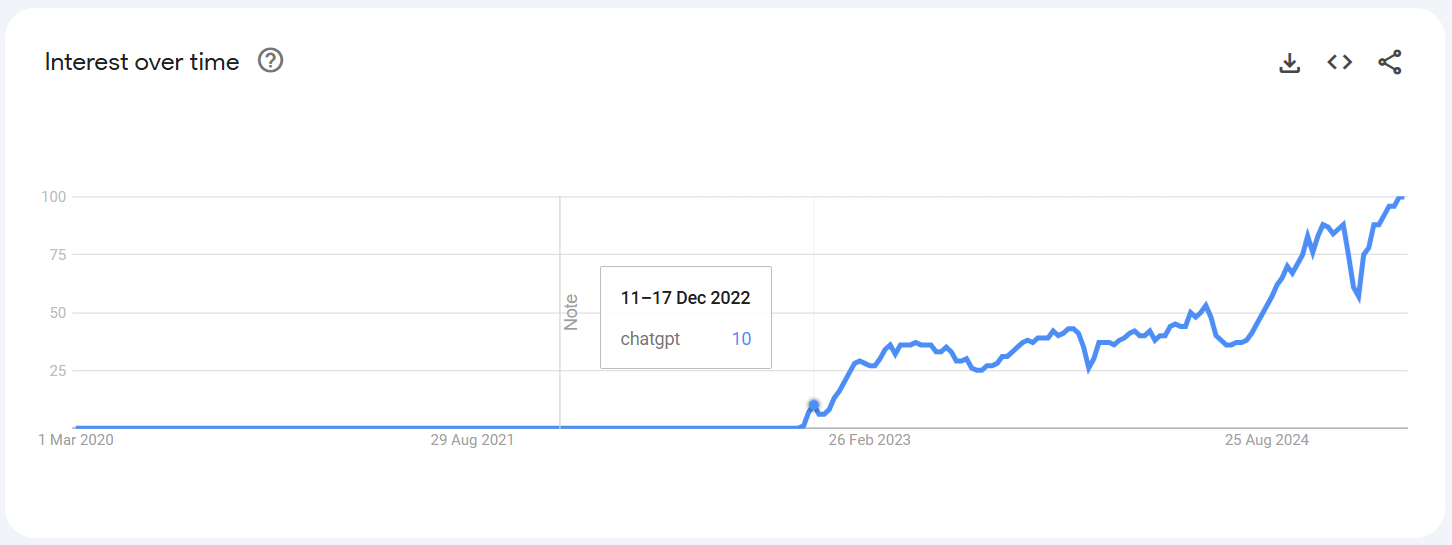
\includegraphics[width=0.9\textwidth]{chatgpt_google_trends.png}
    \caption[Populariteit van de zoekterm ``chatGPT'']{\label{fig:chatgpt_google_trends}Populatireit van de zoekterm ``chatGPT'' op Goole Trends. De interesse blijft maar stijgen naargelang de tijd vordert.}
\end{figure}

Deze doorbraak in \acrlong{AI} heeft \acrfull{LLM} en, in bredere zin, \acrfull{NLP} in de schijnwerpers gezet. \acrshort{NLP} kan worden gedefinieerd als ``de tak van \acrlong{AI} die computers helpt menselijke taal te begrijpen, interpreteren en manipuleren'' \autocite{Zohuri2022}. Het omvat een reeks technieken die het mogelijk maken voor computers om op een natuurlijke manier te communiceren met mensen. \acrshort{LLM}'s daarentegen zijn intelligente systemen die, door gebruik te maken van \acrshort{NLP}-technieken, in staat zijn om tekst te verwerken en te genereren met samenhangende communicatie. 

\acrlong{LLM} zijn zeer diepe kunstmatige neurale netwerken. Lange tijd werden \acrshort{LLM}'s geïmplementeerd met behulp van recurrente neurale netwerken of hun uitbreiding, langetermijngeheugennetwerken \autocite{Delobelle2020}. De transformerarchitectuur, geïntroduceerd door \textcite{Vaswani2017}, bracht hier verandering in: \acrshort{LLM}'s gebouwd op de transformerarchitectuur werden de nieuwe norm en het recurrente gedeelte werd losgelaten. De meerderheid van de huidige \acrshort{LLM}'s rusten vandaag op deze architectuur.

In 2018 publiceerde het bedrijf OpenAI het paper \emph{Improving Language Understanding by Generative Pre-Training} \autocite{Radford2018}. Dit paper adresseerde tekortkomingen die iedere \acrshort{LLM} destijds had. Tot op dat moment werden \acrshort{LLM}'s getraind met behulp van \gls{label}. Aangezien een \acrshort{LLM} enorme hoeveelheden data vereist, kan het labelen van data zeer tijdrovend zijn. Daarnaast zijn er domeinen die schaars zijn aan data. Dit betekent dat, hoewel het labelen van alle beschikbare data mogelijk is, dit weinig zin heeft, aangezien de totale hoeveelheid data niet groot genoeg is om een \acrshort{LLM} effectief te trainen. Uiteindelijk, vertegenwoordigen zelfs volledig gelabelde datasets slechts een deelverzameling van een taal, waardoor niet alle nuances van taal kunnen worden vastgelegd.

\textcite{Radford2018} realiseerden zich het grote potentieel van het benutten van ongelabelde data om de bovengenoemde tekortkomingen aan te pakken, wetende dat de omvang van ongelabelde data groter is dan die van gelabelde data. Ze boden hiervoor een oplossing die gebruikmaakte van unsupervised pre-training op de niet-gelabelde data en supervised fine-tuning op de gelabelde data. Deze techniek noemden ze \emph{\textbf{G}enerative \textbf{P}re-\textbf{T}raining}.

Deze paper zette de nieuwe norm voor de volgende generaties \acrshort{LLM}'s en startte de GPT-revolutie.
 
Zodat de lezer een idee kan krijgen van wat er allemaal verbogen staat achter moderne \acrshort{LLM}'s, geven we hier een bondig samenvatting dat gebaseerd is op \textcite{Naveed2023}.

Elke moderne \acrshort{LLM} heeft volgende basiscomponenten: 
\begin{itemize} 
    \item \textbf{Tokenisatie}: Dit is een pre-processing stap dat training voorgaat. Hier, wordt de invoer onderverdeelt in tokens. Een token kan een character, stuk woord, symbool of woord zijn afhankelijk van de tokenisatie-techniek dat gebruikt wordt.
    \item \textbf{Aandacht}: Deze component wijst gewichten toe aan de input tokens zodat de model meer aandacht richt aan de belangrijkste tokens.
    \item \textbf{Positionele encodering}: Hier wordt informatie toegevoegd met betrekking tot de posities van de tokens. Dit component werkt heel nauw samen met de aandacht zodat de model de invoer begrijpt. Anders uitgedrukt, worden via aandacht de belangrijkste tokens geïdentificieert en via positionele encodering wordt de volgorde en context van deze tokens verstaan.
    \item \textbf{Activatiefunctie}: Deze functies laten toe niet-lineaire relaties aan te leren, wat cruciaal is om met taal aan de slag te gaan.
\end{itemize}

De training van moderne \acrshort{LLM}'s gebeurt in drie fases \autocite{Bach2024}:
\begin{enumerate} 
    \item \textbf{Self-supervised learning} (komt overeen met unsupervised pre-training van \textcite{Radford2018}): In deze stap moet de LLM, gegeven een zin met een ontbrekend woord (of woorden), een lijst genereren van mogelijke woorden die zouden kunnen passen. Deze lijst is gerangschikt op basis van waarschijnlijkheid. Het doel van deze fase is dat het model de eigenschappen van de taal leert begrijpen, evenals de specifieke kenmerken van het datadomein.
    \item \textbf{Supervised learning} (komt overeen met supervised fine-tuning van \textcite{Radford2018}): Hier wordt het model getrained om taken uit te voeren. Voorbeelden van dergelijke taken zijn het genereren van code, het samenvatten van teksten en het beantwoorden van specifieke vragen, om er maar enkele te noemen. Het doel van deze fase is ervoor te zorgen dat het model daadwerkelijk nuttige taken kan uitvoeren in plaats van simpelweg woorden te raden.
    \item \textbf{Reinforcement learning} (is een nieuwe innovatie sinds \textcite{Radford2018}): In deze stap worden de gewenste gedragen aan het model aangeleerd. Dit gebeurt door gewenst gedrag te belonen en ongewenst gedrag te bestraffen.
\end{enumerate}

De indrukwekkende prestaties van \acrshort{LLM}'s in een reeks van taken \autocite{Naveed2023} zijn te danken aan de hedendaagse rekenkracht, de enorme hoeveelheid beschikbare data (voortgebracht door sociale media en het \emph{Internet of Things}), en de groeiende interesse in dit domein \autocite{Zohuri2022, Naveed2023}. Hierdoor zijn \acrshort{LLM}'s uitermate geschikt als basis voor de ontwikkeling van Eureka. 

\section{\IfLanguageName{dutch}{Ontwerp}{Design}}%
\label{sec:ontwerp}

\subsection{\IfLanguageName{dutch}{Specialiseren van LLM's}{Specializing LLM's}}%
\label{subsec:specialiseren_llm}

In 2021 definieerden \textcite{Bommasani2021} het concept van een \emph{foundation model} als ``eender welk model dat is getraind op brede datasets (meestal met grootschalige self-supervision) en dat kan worden aangepast (bijvoorbeeld via fine-tuning) voor een breed scala aan taken''. Met andere woorden, een foundation model is een \acrshort{LLM} dat op een enorme hoeveelheid data is getraind en zo klaargeleverd wordt voor gebruik. Foundationmodellen worden dus kant-en-klaar geleverd met de kennis die ze tijdens hun training hebben verworven.

Gebaseerd op bovenstaande definitie is iedere \acrshort{LLM} die vandaag publiek beschikbaar is, een foundation model. Het probleem hierbij is dat wij een chatbot willen ontwikkelen, gebaseerd op een foundation model, die vragen over vakken \emph{gegeven aan HOGENT} kan beantwoorden. Dit betekent dat onze model extra gespecialiseerde kennis moet bezitten bovenop de reeds verworven kennis tijdens de training.

Om een foundation model te specialiseren, zijn er drie benaderingen mogelijk: werken met het volledige foundation model, een deel van een bestaand model fine-tunen, of de kennis van het model uitbreiden met behulp van \emph{context-injectie}.

De eerste benadering houdt in dat we zelf een \acrshort{LLM} vanaf nul bouwen of herbouwen. Het eerste geval betekent dat we een model vanaf nul ontwerpen en trainen op door ons aangeleverde data. Het tweede geval houdt in dat we alle gewichten van het model aanpassen, zodat het model zich verder specialiseert in de gewenste vaardigheden. Dit wordt in feite beschouwd als het volledig fine-tunen van het model.

Deze eerste benadering is echter niet haalbaar vanwege de aanzienlijke middelen, expertise \autocite{Naveed2023} en tijd die hiervoor nodig zijn. \textcite{Fourrier2024} somt verschillende open-source \acrshort{LLM}'s op, waarvan de meeste meer dan één miljard parameters bevatten. Het is duidelijk dat het trainen van een model met één miljard parameters veel tijd kost en dat het ontwikkelen van een dergelijk model ook een hoog niveau van expertise vereist. Als bewijs voor deze stelling verwijzen we naar \textcite{Chiang2023}, die een \acrshort{LLM} ontwikkelden door een volledig foundation model te fine-tunen. Om aan hun criteria te voldoen, maakten ze gebruik van acht \emph{A100}-GPU’s, waarbij elke trainingssessie ongeveer 300 dollar kostte.

Bovendien, zoals eerder vermeld, heeft een \acrshort{LLM} een enorme hoeveelheid data nodig om effectief te kunnen leren. Op dit moment beschikken we niet over vakgerelateerde data van een dergelijke omvang om dit te realiseren.

Bij de tweede benadering wordt een bestaande \acrshort{LLM} gebruikt, waarbij een deel van de gewichten worden aangepast om het model te specialiseren voor het specifieke doel waarvoor we deze nodig hebben.

Een van de meest gekende technieken is \acrfull{LoRA}. Zo hebben \textcite{Azam2024} PharmaLLM kunnen ontwikkelen, een chatbot die vragen over medicijnen kan beantwoorden en aanwijzingen kan geven aan gebruikers. Dit model werd ontworpen door het Llama 2-model te fine-tunen met behulp van \acrshort{LoRA}. 

\textcite{Hu2024} legt uit dat \acrshort{LoRA} een fine-tuningtechniek is die vertrekt vanuit de volgende vraagstelling: \emph{Bij het specialiseren van een \acrshort{LLM}, is het echt nodig om iedere parameter te fine-tunen?}. Bij deze methode worden de initiële gewichten van het model bevroren, en worden twee kleinere aanpasbare matrices $A$ en $B$ aan het model toegevoegd. De parameters van deze matrices worden willekeurig geïnitialiseerd en uitsluitend zij worden gefinetuned. Na het fine-tuningproces worden de aangepaste gewichten berekend als: \[W' = W + AB\] waarbij $W$ de oorspronkelijke, bevroren gewichten voorstelt, $A$ en $B$ de kleine, getrainde LoRA-matrices zijn en $W'$ de uiteindelijke gewichten na fine-tuning zijn. 

Hieruit blijkt dat \acrshort{LoRA} de oorspronkelijke gewichten niet vervangt, maar eerder een optelling uitvoert met een toegevoegde aanpassing $AB$. Hierdoor kan het model zich specialiseren zonder dat het volledige model opnieuw getraind moet worden. Er zijn dus aanzienlijk minder middelen vereist dan de eerste benadering.

Hoewel de tweede benadering haalbaarder lijkt, blijft de benodigde computationele kracht hoog, waardoor ook de financiële vereisten aanzienlijk zijn. \textcite{Hu2021} hebben dankzij \acrshort{LoRA} de benodigde \emph{VRAM} kunnen laten dalen van 1.5TB naar 350GB bij de fine-tuning van het GPT-3 175B-model.

De GeForce RTX 4060 Ti, met 8GB VRAM (evenveel als de GPUs op het VIC), heeft op 7 maart 2025 een kostprijs van 479,00 €. Indien we iets vergelijkbaars willen doen als \textcite{Hu2021}, zouden we $350GB / 8GB$ $\approx 44$ GPU's nodig hebben, wat neerkomt op een totale kostprijs van $44 \times 479.00 € = 21 076.00 €$.

Bovendien is er, om de juiste fine-tuningtechniek te kiezen --- LoRA is niet de enige techniek --- en het model optimaal te fine-tunen, opniew expertise vereist.

De laatste benadering maakt gebruik van een techniek die we context-injectie zullen noemen. Elk \acrshort{LLM} beschikt over een \emph{contextvenster}. Dit venster bepaalt hoeveel tokens het model als input kan verwerken bij het genereren van een antwoord. Het doel van context-injectie is om de benodigde informatie, waarover de \acrshort{LLM} initieel niet beschikt omdat deze niet in de trainingsdata zat, met betrekking tot de gestelde vraag toe te voegen (met andere woorden, injecteren) op het moment dat het model een antwoord genereert. De informatie over de vakken wordt opgeslagen in een databank. Afhankelijk van de gestelde vraag halen we alleen de relevante informatie op. Met deze benadering kunnen we een bestaande LLM gebruiken zonder een trainingsfase, wat resulteert in lagere middelen en expertise die gemakkelijker toegankelijk is. Context-injectie samen met de data vanuit een databank ophalen is wat men \acrfull{RAG} noemt. Figuur~\ref{fig:rag_simple} schets de werking van \acrshort{RAG} uit. 

\begin{figure}
    \centering
    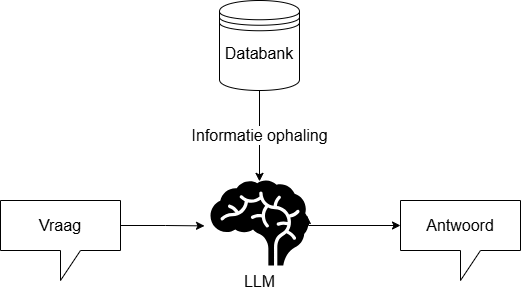
\includegraphics[width=0.8\textwidth]{rag_simple.png}
    \caption[Schets van RAG]{\label{fig:rag_simple}Een eenvoudige schets van de werking van \acrshort{RAG}: de \acrshort{LLM} haalt de benodigde informatie uit een databank om de vraag te beantwoorden.}
\end{figure}

De laatste benadering is de meest veelbelovende met betrekking tot onze onderzoeksdoelstellingen. Ze vraagt minder middelen en vereist geen vakexpertise om te benutten. We onderzoeken deze piste verder.

\subsection{Retrieval-augmented-generation}%
\label{subsec:rag}

In 2020 maakten \textcite{Lewis2020} de volgende vaststelling: LLM's zijn zeer geschikt om diepe inzichten te verkrijgen uit de data waarop ze getraind zijn. Hierdoor hebben ze geen externe \emph{knowledge bases} nodig om vragen te beantwoorden; hun vergaarde kennis fungeert als een impliciete knowledge base. Echter brengt dit enkele uitdagingen met zich mee. Ten eerste is het moeilijk om bestaande kennis te actualiseren zonder het leerproces volledig opnieuw te starten. Dit vormt een tijdrovend proces wanneer frequente updates noodzakelijk zijn. Daarnaast hebben LLM's moeite om vragen te beantwoorden over gebeurtenissen die zich hebben voorgedaan na hun laatste trainingssessie, aangezien ze deze kennis niet bezitten. Dit kan leiden tot hallucinaties \autocite{Gao2023}.

Om deze beperkingen aan te pakken, introduceerden de auteurs een nieuwe techniek genaamd Retrieval-Augmented Generation (RAG). Bij deze techniek wordt een vraag beantwoord door aanvullende kennis op te halen uit externe bronnen en deze te gebruiken om een antwoord te genereren. Zoals \textcite{Lewis2020} het omschrijven: ``De invoersequentie $x$ wordt gebruikt om tekstdocumenten $z$ op te halen, die vervolgens dienen als aanvullende context bij het genereren van de doelsequentie $y$''.

Alle RAG-systemen bestaan uit drie belangrijke stappen \autocite{Gao2023}:  

\begin{enumerate} 
    \item \textbf{Indexing}: Hier wordt ruwe data uit verschillende formaten (bijvoorbeeld PDF, HTML, DOCX) opgehaald. Vervolgens wordt deze data geconverteerd naar tekst en opgeschoond. Belangrijk hierbij is dat de tekst wordt opgedeeld in brokken. De reden hiervoor is dat het contextvenster van LLM's een beperkte grootte heeft, waardoor het beter is om alleen de relevante brok door te geven in plaats van het gehele document, waarbij het risico bestaat dat niet alles past. Bovendien is uit onderzoek gebleken dat LLM's meer aandacht besteden aan het begin en einde van het contextvenster en minder aan het midden. Dit fenomeen staat bekend als het \emph{lost in the middle}-fenomeen \autocite{Databricks}. Daarom is het beter om kleinere contexten door te geven dan grote, zodat de aandacht van de LLM behouden blijft. Uiteindelijk, worden de brokken opgeslaan in een databank; de ruwe data wordt zo geïndexeerd. 
    \item \textbf{Retrieval}: In deze fase wordt de gebruikersinvoer omgezet naar hetzelfde indexformaat als in de vorige stap. Zodra de invoer in hetzelfde formaat is, kunnen we de relevante brokken ophalen waarmee we het contextvenster verrijken.   
    \item \textbf{Generation}: Tot slot wordt het finale antwoord gegenereerd. Merk op dat de \acrshort{LLM} voornamelijk wordt gebruikt voor haar taalcapaciteiten bij het formuleren van het antwoord. Het grootste deel van het werk wordt echter uitgevoerd in de twee voorgaande fases.
\end{enumerate}

In wat volgt bespreken we de twee eerste stappen meer in detail.

\subsubsection{Indexing}%
\label{subsubsec:indexing}

De indexing stap kan onderverdeelt worden in drie fases.

De eerste fase bestaat uit het ophalen van ruwe data uit bestanden van verschillende formaten, zoals PDF, HTML of DOCX. Dit betekent dat alle overbodige metadata die bij deze formaten horen, worden verwijderd, zodat alleen de ruwe tekst overblijft. Daarnaast kan worden bepaald in hoeverre de tekst ruw moet zijn. Er kunnen extra stappen worden uitgevoerd om de structuur van de lay-out te behouden, bijvoorbeeld door aan te geven waar titels stonden, welke delen tot een tabel behoorden, enz.

De tweede fase bestaat uit het verdelen van de ruwe data in brokken. Zoals eerder aangegeven, is het contextvenster van een \acrshort{LLM} beperkt. Aangezien de prompt die aan de \acrshort{LLM} wordt gevoerd extra context zal bevatten (contextinjectie), mag deze context niet te lang zijn. Anders bestaat het risico dat niet alles in het contextvenster past, waardoor de \acrshort{LLM} niet correct of volledig op vragen kan antwoorden. Daarom is deze fase essentieel en van uitermate groot belang.

De manier waarop brokken worden aangemaakt, hangt af van de toepassing; er bestaat geen universele techniek om dit correct te doen. Toch bestaan er verschillende technieken, die \textcite{Kshirsagar2024} heeft verzameld en die wij hier zullen opsommen:

\begin{enumerate} 
    \item \textbf{Vaste lengte brokken}: deze techniek is het eenvoudigste: de documenten worden onderverdeelt in brokken van vaste lengte $n$. Deze techniek is ook het minst vragende sinds er geen aandacht moet besteed worden aan de semantiek. 
    
    Er wordt aangeraden om vaste lengte brokken te gebruiken wanneer de brok grootte belangrijker is dan de semantiek.
    \item \textbf{Content-Aware Chunking}: deze familie van technieken zijn complexer dan de vorige techniek. Hier, wordt aandacht besteed aan het behouden van de semantische samenhang binnen iedere brok.
    
        \begin{itemize}
            \item \textbf{Recursive chunking}: Hier wordt getracht brokken te creëren die niet groter zijn dan $n$. Dit gebeurt door de tekst op te splitsen volgens een voorkeursvolgorde. Er wordt enkel naar het volgende niveau gegaan als de brok nog steeds groter is dan $n$: eerst op paragraafniveau, daarna op zinsniveau, vervolgens op spaties, en uiteindelijk op individuele tekens.
            
            De resulterende brokken hebben niet noodzakelijk exact dezelfde grootte, maar hun omvang blijft vergelijkbaar,
            \item \textbf{Sentence-Aware Chunking}: Bij deze techniek wordt ervoor gezorgd dat er niet midden in een zin wordt gesneden. Een brok bevat dus altijd volledige zinnen. Daarnaast wordt erop gelet dat een brok niet langer wordt dan $n$
            \item \textbf{Semantic chunking}: Deze techniek is de meest geavanceerde, omdat deze de interventie van een LLM met embedding-capaciteiten vereist. Daarnaast richt deze techniek zich puur op semantiek, in tegenstelling tot de twee voorgaande technieken, die dit slechts indirect proberen te benaderen door zich te baseren op zinssamenhang. 
            
            Hierbij wordt het document eerst verdeeld in zinnen. Elke zin wordt vervolgens voorgesteld als een vector met behulp van de LLM-embedding. Aan de hand van wiskundige berekeningen (zie~\ref{subsubsec:retrieval}) worden zinnen met dezelfde semantische betekenis gegroepeerd. Deze groepen vormen uiteindelijk de brokken.
        \end{itemize}
\end{enumerate}

Ten slotte, is de laatste fase het indexeren, oftewel het opslaan van de brokken in de databank. De manier waarop dit gebeurt, hangt af van de volgende stap, met andere woorden, van de \emph{retrieval-strategie}. 

\subsubsection{Retrieval}%
\label{subsubsec:retrieval}
In deze stap wordt de relevante informatie (brokken) uit de databank opgehaald en doorgevoerd naar de \acrshort{LLM}. De manier waarop de brokken worden opgehaald in relatie tot de invoerquery van de gebruiker, hangt af van de onderliggende retrieval-strategie, en dus van de gebruikte databanktechnologie.

De eerste strategie is keyword-search \autocite{Bansal2023}. Hierbij worden brokken opgehaald op basis van exacte keyword matches. Als er bijvoorbeeld gevraagd wordt ``Wanner is het examen van DSAI'', dan wordt er gezocht precies gezocht op de keywords ``examen van DSAI''. Indien er zuiver voor deze strategie wordt gekozen, kan de databank een gewone databank zijn; de brokken worden dus als plain text opgeslaan. De gebruikte algoritme hier is \emph{BM25} \autocite{Bansal2023}.

Deze strategie is bijzonder effectief wanneer er zeer gespecialiseerde woorden of niche-termen worden gebruikt die onwaarschijnlijk voorkomen in de datasets waarmee \acrshort{LLM}'s zijn getraind.

De tweede strategie is Vector Search \autocite{Bansal2023}. Hierbij worden de brokken opgeslagen in een vectorvoorstelling. Om deze vectorvoorstelling te verkrijgen, worden embeddingmodellen gebruikt die zijn getraind om zinnen zo optimaal mogelijk om te zetten in een vector, rekening houdend met de gebruikte taal. Met andere woorden, er zit een bepaalde semantische logica achter de vectoren.

Brokken worden opgehaald op basis van hun verband met de invoer. Hiervoor wordt de invoer van de gebruiker eerst omgezet naar een vectorvoorstelling, gebruikmakend van hetzelfde embeddingmodel als bij het indexeren van de brokken. Vervolgens wordt de inputvector vergeleken met de geïndexeerde brokken aan de hand van een afstandsmetric. Deze metric is meestal de cosinusgelijkenis. De brokken die worden opgehaald, zijn die waarvan de afstand het kleinst is ten opzichte van de inputvector.

Figuur~\ref{fig:vector_search} toont een vereenvoudigde illustratie van vector search in het cartesisch coördinatenstelsel. Hierbij zien we de ge-embedde invoer van de gebruiker, voorgesteld als een cirkel. Daarnaast zien we de ge-embedde brokken, voorgesteld als documenten. Aan de hand van de afstandsmetric wordt bepaald welke brokken waarschijnlijk het meest relevant zijn voor de invoer. In dit geval zijn er twee brokken die zich het dichtst bij de invoer bevinden. Omdat deze brokken de kleinste afstand tot de input hebben, worden ze geretourneerd als relevante context.

\begin{figure}
    \centering
    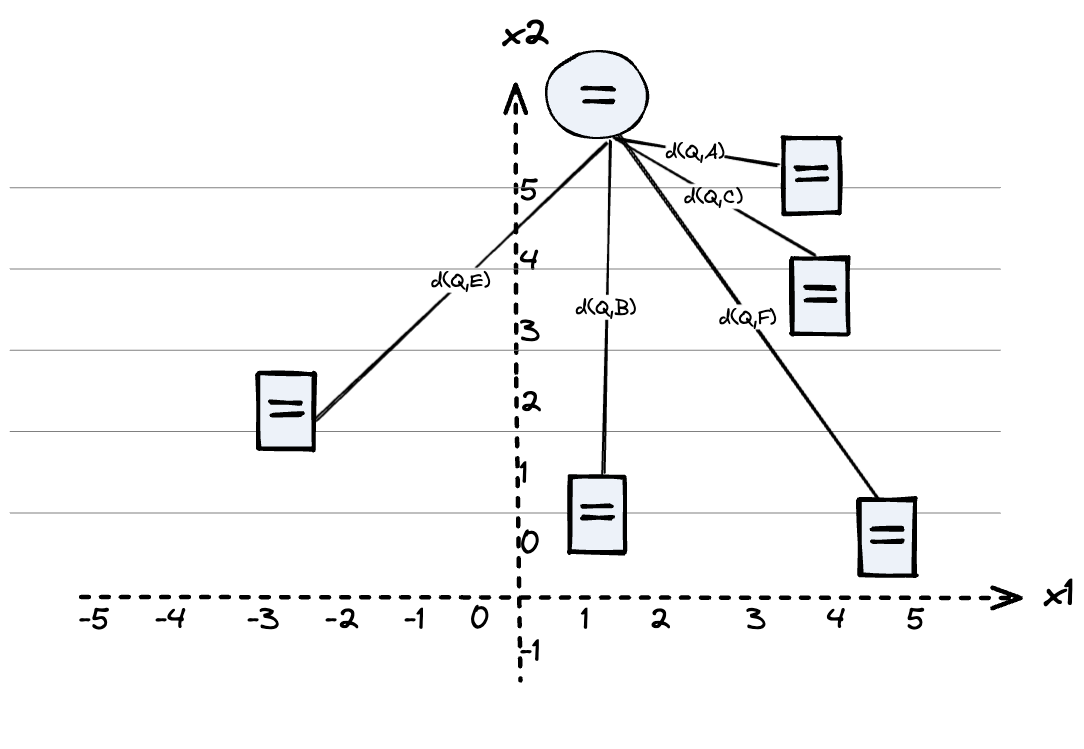
\includegraphics[width=0.8\textwidth]{vector_search.png}
    \caption[Vulgarisatie van Embbe Search in het cartesisch coördinatenstelsel]{\label{fig:vector_search}Een vereenvoudigde illustratie van Vector Search. De cirkel stelt de gebruikersinput en de documenten stellen de verschillende brokken voor \autocite{Vespa2023}.}
\end{figure}
        
Deze tweede strategie is bijzonder effectief in het begrijpen van de betekenis achter queries, zelfs wanneer de gebruikte woorden niet exact overeenkomen. Met andere woorden, vector search is zeer geschikt voor het vinden van semantisch gerelateerde woorden.

Indien er puur voor deze strategie wordt gekozen, moet de gebruikte databank een \emph{vectordatabank} zijn. Dergelijke databanken ondersteunen zowel het opslaan van embeddings als het opzoeken van vectoren.

De laatste strategie is Hybrid Search \autocite{Bansal2023}. Hierbij worden de beste aspecten van beide werelden gecombineerd tot één strategie. Deze methode stelt RAG-systemen in staat om informatie op te halen die zowel de juiste woorden als de juiste betekenis bevat. 

\subsection{\IfLanguageName{dutch}{Valkuilen}{Pitfalls}}%
\label{subsec:valkuilen}

Bij het ontwerpen van Eureka zijn er twee belangrijke valkuilen die bijzondere aandacht vereisen: \textbf{onverwachte interacties} en \textbf{hallucinaties}.

Tijdens de ontwikkeling van de chatbot \emph{LiSA} constateerden \textcite{Dibitonto2018} dat er een tendens bestond om LiSA te antropomorfiseren, ondanks haar beperkte complexiteit. Dit resulteerde in onverwachte reacties, zoals uitingen van dankbaarheid of het gebruik van smileys om zinnen te benadrukken. Helaas leidde dit ook tot ongepast gedrag; sommige gebruikers reageerden agressief of gaven de interactie een seksuele connotatie. Onverwachte interacties kunnen echter niet alleen voortkomen uit gebruikers, maar ook uit de chatbot zelf.

Een voorbeeld hiervan is \emph{Prompt Hacking}, een aanvalsmethode waarbij specifieke prompts worden ingevoerd met als doel de LLM gedrag te laten vertonen dat afwijkt van de oorspronkelijke bedoeling van het model \autocite{Rababah2024}. Dergelijk afwijkend gedrag kan bijvoorbeeld bestaan uit het openbaar maken van privé-informatie of het maken van beledigende opmerkingen \autocite{Naveed2023}.

Daarnaast is vastgesteld dat LLM's onderhevig kunnen zijn aan een fenomeen dat bekend staat als \emph{hallucinatie}. Hierbij genereert de LLM coherente uitvoer die echter gebaseerd is op onjuiste informatie. Dit fenomeen kan worden onderverdeeld in drie categorieën \autocite{Naveed2023}:

\begin{itemize} 
    \item \textbf{Input-conflicterende hallucinatie}: de gegenereerde output heeft weinig tot geen verband met de ingevoerde gegevens. 
    \item \textbf{Context-conflicterende hallucinatie}: de gegenereerde output is in tegenspraak met eerder gegenereerde output. 
    \item \textbf{Feit-conflicterende hallucinatie}: de output bevat onjuiste informatie over algemeen bekende feiten (bijvoorbeeld: ``Parijs is de hoofdstad van Pakistan''). 
\end{itemize}

Hallucinaties dienen strikt vermeden te worden bij het ontwerpen van Eureka, aangezien ze het risico met zich meebrengen om meer verwarring te zaaien in plaats van duidelijkheid te bieden.

\textcite{Taneja2024} stelt een raamwerk voor om dit probleem te mitigeren.

Voor hallucinatie wordt het model gevraagd om eerlijk te zijn. Indien het niet in staat is om een vraag te beantwoorden op basis van de gegeven context, moet het dit gewoon toegeven. Dit zeer eenvoudige mechanisme vermindert hallucinaties, omdat er niet slechts één enkele optie is (waarbij het model per se iets moet genereren), maar ook een alternatieve optie: erkennen dat het geen voldoende informatie heeft.

Voor onverwachte interacties wordt het model gevraagd om de invoer te categoriseren op basis van zijn \emph{skills}. Deze skills zijn:

\begin{itemize}
    \item \textbf{De zelfbewustzijnsskill}: Onder deze categorie vallen vragen over het model zelf. Het model kan bij dergelijke vragen altijd eenzelfde generiek antwoord geven.
    \item \textbf{De begroetingsskill}: Onder deze skill vallen begroetingen van gebruikers. Het model kan hier zonder problemen op reageren.
    \item \textbf{De beantwoording skill}: Hieronder vallen alle vragen met betrekking tot vakken. Zodra een dergelijke vraag binnenkomt, wordt het RAG-proces in gang gezet.
\end{itemize}

Elke vraag die niet binnen deze skills valt, wordt vriendelijk geweigerd.

Daarnaast wordt de \emph{Moderation API} van OpenAI gebruikt om onaanvaardbare invoer te detecteren. Dit is met name nuttig in gevallen waarin Prompt Hacking wordt toegepast om het skill-based raamwerk te omzeilen.

Het gebruik van de API is gratis.

\section{\IfLanguageName{dutch}{Besluit}{Conclusion}}%
\label{sec:besluit}

Uit de literatuurstudie blijkt dat een chatbot een geschikte oplossing biedt om een centrale plaats te creëren waar studenten en docenten op een interactieve manier hun vragen kunnen stellen en on-demand een antwoord kunnen ontvangen.

Chatbots zijn een technologie die al geruime tijd bestaat en oorspronkelijk voornamelijk gebaseerd was op patroonherkenning. Met de vooruitgang in \acrshort{NLP} en, meer specifiek, in \acrshort{LLM}'s, kunnen we nu flexibelere chatbots ontwikkelen die niet langer afhankelijk zijn van strikt gedefinieerde regels. Het zelf ontwikkelen van een \acrshort{LLM}, of fine-tunen ervan, valt echter buiten de scope van dit onderzoek en overschrijdt de beschikbare middelen. Daarom is besloten om een bestaande \acrshort{LLM} te gebruiken.

Aangezien bestaande \acrshort{LLM}'s vaak worden geleverd met vooraf vergaarde kennis, maar wij gespecialiseerde kennis nodig hebben, is het noodzakelijk om de kennis van de \acrshort{LLM} uit te breiden met externe bronnen.

Om dit te realiseren, zal gebruik worden gemaakt van RAG, een techniek die specifiek is ontworpen voor dit doel. Bovendien is RAG bijzonder geschikt voor de dynamische omgeving van het onderwijs, die vaak verandert. Daarnaast is het een gebruiksvriendelijkere oplossing voor ons doelpubliek, dat niet per se vakexperten zijn, dan het direct aanpassen van een \acrshort{LLM}.

Bij het ontwerp van Eureka zal er bovendien aandacht besteed moeten worden aan de valkuilen die voortkomen uit de menselijke natuur. Eureka moet voorbereid zijn op onverwachte interacties en situaties. Hierbij zullen we gebruik maken van de raamwerk van \textcite{Taneja2024}.

% Tip: Begin elk hoofdstuk met een paragraaf inleiding die beschrijft hoe
% dit hoofdstuk past binnen het geheel van de bachelorproef. Geef in het
% bijzonder aan wat de link is met het vorige en volgende hoofdstuk.

% Pas na deze inleidende paragraaf komt de eerste sectiehoofding.

%Dit hoofdstuk bevat je literatuurstudie. De inhoud gaat verder op de inleiding, maar zal het onderwerp van de bachelorproef *diepgaand* uitspitten. De bedoeling is dat de lezer na lezing van dit hoofdstuk helemaal op de hoogte is van de huidige stand van zaken (state-of-the-art) in het onderzoeksdomein. Iemand die niet vertrouwd is met het onderwerp, weet nu voldoende om de rest van het verhaal te kunnen volgen, zonder dat die er nog andere informatie moet over opzoeken \autocite{Pollefliet2011}.
%
%Je verwijst bij elke bewering die je doet, vakterm die je introduceert, enz.\ naar je bronnen. In \LaTeX{} kan dat met het commando \texttt{$\backslash${textcite\{\}}} of \texttt{$\backslash${autocite\{\}}}. Als argument van het commando geef je de ``sleutel'' van een ``record'' in een bibliografische databank in het Bib\LaTeX{}-formaat (een tekstbestand). Als je expliciet naar de auteur verwijst in de zin (narratieve referentie), gebruik je \texttt{$\backslash${}textcite\{\}}. Soms is de auteursnaam niet expliciet een onderdeel van de zin, dan gebruik je \texttt{$\backslash${}autocite\{\}} (referentie tussen haakjes). Dit gebruik je bv.~bij een citaat, of om in het bijschrift van een overgenomen afbeelding, broncode, tabel, enz. te verwijzen naar de bron. In de volgende paragraaf een voorbeeld van elk.
%
%\textcite{Knuth1998} schreef een van de standaardwerken over sorteer- en zoekalgoritmen. Experten zijn het erover eens dat cloud computing een interessante opportuniteit vormen, zowel voor gebruikers als voor dienstverleners op vlak van informatietechnologie~\autocite{Creeger2009}.
%
%Let er ook op: het \texttt{cite}-commando voor de punt, dus binnen de zin. Je verwijst meteen naar een bron in de eerste zin die erop gebaseerd is, dus niet pas op het einde van een paragraaf.
%
%\begin{figure}
%  \centering
%  
\includegraphics[width=0.8\textwidth]{grail.jpg}
%  \caption[Voorbeeld figuur.]{\label{fig:grail}Voorbeeld van invoegen van een figuur. Zorg altijd voor een uitgebreid bijschrift dat de figuur volledig beschrijft zonder in de tekst te moeten gaan zoeken. Vergeet ook je bronvermelding niet!}
%\end{figure}
%
%\begin{listing}
%  \begin{minted}{python}
%    import pandas as pd
%    import seaborn as sns
%
%    penguins = sns.load_dataset('penguins')
%    sns.relplot(data=penguins, x="flipper_length_mm", y="bill_length_mm", hue="species")
%  \end{minted}
%  \caption[Voorbeeld codefragment]{Voorbeeld van het invoegen van een codefragment.}
%\end{listing}
%
%\lipsum[7-20]
%
%\begin{table}
%  \centering
%  \begin{tabular}{lcr}
%    \toprule
%    \textbf{Kolom 1} & \textbf{Kolom 2} & \textbf{Kolom 3} \\
%    $\alpha$         & $\beta$          & $\gamma$         \\
%    \midrule
%    A                & 10.230           & a                \\
%    B                & 45.678           & b                \\
%    C                & 99.987           & c                \\
%    \bottomrule
%  \end{tabular}
%  \caption[Voorbeeld tabel]{\label{tab:example}Voorbeeld van een tabel.}
%\end{table}

